\documentclass[a4paper,twoside]{article}
\usepackage[T1]{fontenc}
\usepackage{graphicx,amsmath,booktabs,array,pslatex,apalike}
\usepackage{algorithm2e}
\usepackage[bottom]{footmisc}
\usepackage{url}
\usepackage[hidelinks]{hyperref}
\usepackage{SCITEPRESS}
\graphicspath{{figures/}}
\newcommand{\doi}[1]{\href{https://doi.org/#1}{doi: \nolinkurl{#1}}}
\newcommand{\aicredit}{\footnote{AI assistance in this section: Codex \cite{codex}. See the disclosure.}}
\begin{document}
\title{Overseeing Many LLMs: A Review-and-Release Workflow}
\author{\authorname{Anonymous Submission}}
\keywords{Human-Agent Interaction, Agent Oversight, Review Workflows, Source Context, Computational Simulation.}
\abstract{Concurrent language-model workers can produce answers faster than a person can inspect them. We argue that oversight should treat each output as a versioned review request, preserving its evidence, unresolved status and individual release authority. We implement an asynchronous review desk and analyze when reviewing related outputs consecutively could help. The computational study uses 36 original questions from six real financial-report contexts and genuine saved model drafts, with explicitly simulated reviewer behavior. Across 31,680 runs in 66 declared settings, source grouping exceeds a first-in-first-out queue in 24 setting means but falls below a bounded source-aware queue in 62 and ties it in four. These counts describe designed scenarios, not the prevalence of benefits in practice. Source-orientation savings can improve modeled completion, but grouping overhead, persistent familiarity, carryover errors and weak draft usefulness can offset them. The position is therefore to preserve explicit review and release while testing rich grouping interfaces against simple source-aware navigation. Workflow reliability is implemented and checked; human effectiveness remains to be established.}
\onecolumn\maketitle\normalsize\setcounter{footnote}{0}\vfill

\section{INTRODUCTION}
\label{sec:intro}
Concurrent workers produce new outputs while earlier answers are still being checked. Related questions share evidence but require different calculations. Postponed corrections can lose their context, and revisions can make approval ambiguous. More agent activity does not necessarily produce more work that a user can confidently release.\aicredit

Our position is that concurrent outputs should be managed as \emph{individually reviewable, versioned requests}. The source, proposed answer and requested decision should remain stable during inspection. Unfinished work should remain visible when the user defers a question or pauses new task starts. Related requests may share a view of their evidence, but sharing a source must not merge the authority to approve their answers.

The contribution combines established queueing, batching and version-control mechanisms in an implemented oversight contract. We specify its observable guarantees and computationally separate source-aware navigation from richer grouping. An interface may appear useful simply because it changes the order in which evidence is revisited; we make that alternative explanation explicit.



The analysis finds a conditional benefit of source-aware ordering, but no setting mean favors grouping over the bounded source-aware control. This motivates a stronger comparator for interface research, not a claim that grouped presentation cannot help people.

\section{CLOSEST RELATED WORK}
\label{sec:related}
Agent interfaces already support substantial observation and intervention. AgentGUI provides concurrent agent desks, shared artifacts, activity inspection, steering and restoration of saved workspaces. Its evaluation includes a small within-person study of trajectory lookup and comprehension \cite{agentgui}. AGDebugger provides a message queue with play, step and pause, message editing, state checkpoints and forks for debugging multi-agent execution. Its user studies examine error identification and steering \cite{agdebugger}. These are close predecessors, not empty dashboards against which any central queue would be an advance.\aicredit

Our emphasis is the boundary between inspecting an output and authorizing its release, preserved through arrivals, deferral and revision. We have not compared the interface with these predecessors in a user study or established that all analogous controls are absent. The contribution is the explicit workflow contract and the comparison needed to attribute benefit to source grouping.

Source reconstruction and interruption recovery have established histories. Iqbal and Horvitz studied disruption and recovery in everyday computing, distinguishing returning to an application from resuming its task \cite{iqbal}. Their observations motivate separating orientation from subsequent answer checking. They do not supply calibrated times for financial-question review. Scheduling research likewise studies batches that share setup costs \cite{potts}. Our source-aware queues instantiate simple related ordering ideas, without claiming a batching optimality result. The central question here is whether their benefit survives fallible review and whether a richer presentation adds anything beyond their selection order.



\section{THE REVIEW-AND-RELEASE WORKFLOW}
\label{sec:workflow}
\subsection{Requests, Evidence and Authority}
A task $i$ has an original question, a source identifier $s_i$, and a proposed output $a_{i,v}$ at version $v$. A request records the worker, task and question identifiers, source provenance, arrival time, current status, output history and requested user decision. Explicit dependencies can be registered. Similar wording or a shared source identifier does not establish a dependency or a shared correct answer.\aicredit

The review desk exposes the original table and paragraphs beside the answer and scale, labeling generated explanations and citations as model content. No executable derivation is required. Missing drafts remain requests that can be answered, rejected or deferred.

Figure~\ref{fig:workflow} summarizes the interaction. An offered task is accounted for before it starts. Its generated output is received and queued. Selecting it creates an active snapshot of the exact source and output version. New arrivals update pending work without replacing that snapshot. Optional source sessions expose up to three questions beside their common source, while preserving separate fields and decisions.

\begin{figure*}[t]
\centering
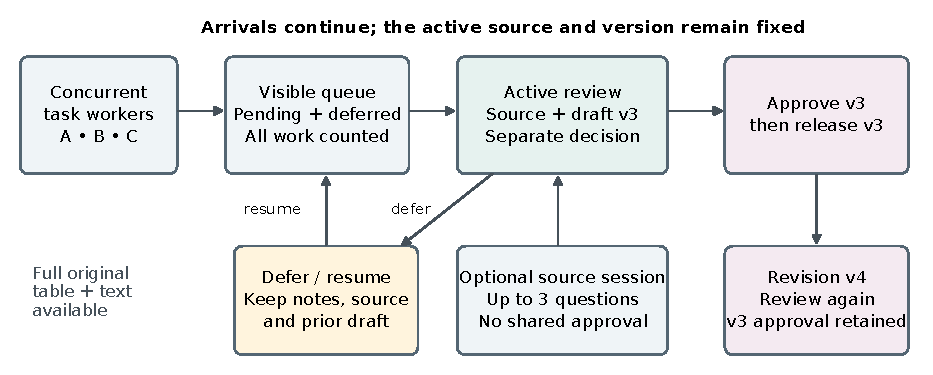
\includegraphics[width=\textwidth]{workflow.pdf}
\caption{Workflow schematic, not a user observation. Arrivals preserve the active source and version; deferral retains notes and drafts. Grouped questions retain individual decisions. Approval of version 3 does not approve version 4. No human timing or comprehension is depicted.}
\label{fig:workflow}
\end{figure*}

Approval, correction, rejection and deferral have distinct effects. Approval marks the inspected version as acceptable but does not release it. Correction creates a new output version and approves that specific replacement. Release is a subsequent explicit command. Rejection blocks the answer and leaves the deliverable incomplete. Deferral preserves notes, source, prior draft and action history for resumption. Withdrawal or supersession is explicit and remains in the accounting.

Separating approval from release allows a user to retain an accepted draft while other work remains unsettled. It also gives the system a precise final check. A release command names the request and version and succeeds only if that version is both current and approved. A later revision preserves the historical approval but requires review again. If the active snapshot has become stale, the desk shows that fact rather than silently substituting the revision. This contract prevents stale authorization within the application; it cannot establish that the reviewed answer is correct.

\subsection{Concurrency and Observable Properties}
The backend serializes state-changing commands under a lock and validates each transition. Repeated delivery of the same command identifier and payload returns the recorded result; conflicting reuse is refused. Invalid transitions roll back. An ordered event history supports deterministic replay of logical state. Live workers and saved-output replay use the same request protocol.

The resulting properties concern application state. Every offered or received item remains accounted for. An arrival cannot alter the active snapshot. Decisions identify exact versions. A revision cannot inherit approval. Deferral retains history, and pausing admission prevents new starts without erasing offered tasks or stopping an in-flight generation. Grouping never creates collective approval authority. The properties assume commands pass through this local single-process controller; they do not cover distributed transactions or external publication rollback.

The software evaluation exercised 144 real-output replay scenarios with compressed arrivals, scripted deferral, admission pauses and revisions: 13,236 events and 41,722 active-review preservation checks, with zero failures of that check. An ideal annotation-based script completed all work under ample scripted capacity. This mechanical tie is not human evidence. A live demonstration used three workers and actual generation arrivals through the same protocol.

\section{COMPUTATIONAL EVALUATION}
\label{sec:model}
\subsection{Real Inputs and Constructed Workloads}
TAT-QA provides financial table-and-text questions \cite{tatqa}. The study reuses 36 original questions from six source contexts, organized into three packets of twelve questions from two sources each. The packets use all questions at zero-based public \texttt{test\_gold} context indices (51,53), (52,38), and (26,28), respectively, in the official repository revision 870accc.\footnote{\url{https://github.com/NExTplusplus/tat-qa/tree/870accc}} These materials had already been inspected during system development; this is not a fresh held-out task evaluation. Context identifiers support grouping, but reliable report-level independence is unavailable. The source tables and text are real financial-report material, the questions are benchmark annotations, and the worker assignments are constructed.\aicredit

Workers are separately prompted tasks sharing one model architecture. Each question uses saved replica 0 from Qwen2.5-7B-Instruct, generated at temperature 0.3 with a 230-token output limit and a 2,048-token context limit. The model provides an answer, scale and optional explanation. The selected set contains seven initially joint-correct drafts and five empty or unsupported displayed answer fields. Joint correctness requires the official answer match and the annotated scale. We retain all questions and these failures. No new inference is used in the simulation or this consolidation.

The larger software collection contains 145 questions from 24 contexts and 290 generations: 61 answer exact matches and originally 38 empty outputs. A uniform pilot projection restored seven parser-lost displays, leaving 31 empty or unsupported fields. Exact match remained 61/290. The simulation uses that display projection on its smaller fixed set; the repair did not improve correctness.

The initial scenario offers twelve questions with a nine-minute cutoff. Task starts occur at 0, 4, 8, 12, 16 and 20 seconds, then at 180, 184, 188, 192, 196 and 200 seconds. Delivery follows each start by 0.25 seconds. Source identifiers alternate in the original order. These times are constructed, not recorded workplace arrivals or model latencies. Rotating the three packets exposes every question without treating rotations as additional source contexts.

\subsection{Policies and Information Boundary}
Table~\ref{tab:policies} defines all five policies. At each selection opportunity, eligible requests are arrived, queued requests or deferrals whose return time has passed. Ties use arrival time and a stable identifier. Review is nonpreemptive. No policy waits deliberately to form a group. All policies have the same source identifiers, available requests and decision authority. They cannot see benchmark correctness, future arrivals or future random outcomes.

\begin{table}[t]
\caption{Simulated navigation policies. Q and M share arrival order. G adds presentation cost to the bounded rule, not privileged evidence.}
\label{tab:policies}
\centering
\begin{tabular}{@{}>{\raggedright\arraybackslash}p{.21\linewidth}>{\raggedright\arraybackslash}p{.725\linewidth}@{}}
\toprule
Policy & Next-review rule \\
\midrule
Q: FIFO & Oldest eligible request, with a saved draft. \\
G: grouping & Start from FIFO, then finish a set of at most three currently available requests from that source. Charge a grouping cost for a multi-question set. \\
Bounded source queue & Identical selection mechanism to G, without grouping cards or their cost. \\
Sticky source queue & Continue with the last reviewed source while an eligible request remains; otherwise FIFO. \\
M: manual & FIFO, with source and question but no model draft or explanation. \\
\bottomrule
\end{tabular}
\end{table}

G and the bounded source queue share the same selector. At zero grouping cost their paired trajectories are identical by construction, not an empirical discovery. The model supplies no measured comprehension benefit for cards. Positive cost can change later eligibility, so the shared selector does not prove universal dominance.

The real central queue permits manual selection. FIFO is a strategy, not an imposed interface restriction. Both source-aware controls represent choices possible without grouped cards. G assumes available groups are used; adoption is not measured.

\subsection{Timing, Familiarity and Fallibility}
A review comprises grouping when applicable, source orientation, question interpretation, verification or construction, and interaction. The base values and ranges are in Table~\ref{tab:parameters}. These are analyst-selected assumptions, not measurements of human financial-review performance.

For a previously visited source, orientation time is
\begin{equation}
 O_s = S f_s \left[r+(1-r)\left(1-e^{-\Delta_s/\tau-k_s/\kappa}\right)\right].
 \label{eq:orientation}
\end{equation}
For an unseen source it is $S f_s$. Here $S$ is an orientation coefficient in seconds, $\Delta_s$ is time since the last completed decision on that source, and $k_s$ counts intervening completed decisions on other sources. The residual fraction $r=0.1$ prevents free reorientation. The time constant $\tau$ and decision constant $\kappa$ govern persistence. All policies share this memory model. Orientation is evaluated after any grouping overhead, at the start of orientation, and is fixed for that attempt. Even an unsuccessful completed review refreshes familiarity. No additional switching cost is charged.

The source factor is $f_s=\min(1.25,\max(0.75,c_s/3200))$ for $c_s$ table-and-paragraph characters. All six sources have 1,120--1,750 characters, hence $f_s=0.75$: $S=25$ means 18.75 seconds for a new source. This clipping removes source-size variation, so the study cannot validate size scaling.

\begin{table}[t]
\caption{Assumed reviewer parameters. The reference uses the higher-effectiveness profile, long memory and the base times. Sensitivities change specified subsets, not every Cartesian combination.}
\label{tab:parameters}
\centering
\begin{tabular}{@{}>{\raggedright\arraybackslash}p{.46\linewidth}>{\raggedright\arraybackslash}p{.475\linewidth}@{}}
\toprule
Quantity & Values \\
\midrule
Orientation coefficient $S$ & 0, 5, 25, 75 s \\
Short memory $(\tau,\kappa)$ & (45 s, 2 decisions) \\
Long memory $(\tau,\kappa)$ & (600 s, 8 decisions) \\
Persistent-memory stress & $(10^{12}$ s, $10^{12})$ \\
Question interpretation & 8 s base \\
Draft verification & 18 s; sensitivity 8, 40 s \\
Detected-error correction & 45 s base \\
Manual or missing draft & 45 s; sensitivity 20, 90 s \\
Grouping per opened set & 4 s; sensitivity 0, 12 s \\
Decision; release & 2 s each \\
Carryover probability & 0; sensitivity 0.08, 0.20 \\
\midrule
Profile: $(d,c,h,m)$ & Detect, correct, damage, manual \\
Ideal & $(1,1,0,1)$ \\
Higher & $(0.85,0.85,0.02,0.75)$ \\
Limited & $(0.55,0.60,0.08,0.50)$ \\
\bottomrule
\end{tabular}
\end{table}

Interpretation, verification and construction times each multiply their base by $1+\min(w_i,40)/80$, where $w_i$ is question length in words, and by a mean-one lognormal draw with log standard deviation 0.2. Orientation and interface costs are not jittered. These functions provide reproducible task variation, not estimated reading times.

For a nonempty wrong draft, detection occurs with probability $d$. Detection adds construction time; correction succeeds with probability $c$. An undetected error is approved incorrectly. An initially correct draft can be damaged with probability $h$, modeled within the verification phase. M and empty drafts take the construction path with success probability $m$. An unsuccessful construction is recognized with probability 0.5. Recognition leads to a 45-second deferral on the first attempt and rejection on the second; an unrecognized failure is released incorrectly. There are at most two attempts. A separate carryover probability can spoil an otherwise correct answer when the immediately preceding completed question used the same source. It applies to all five policies, including manual work.

Annotations determine these simulated outcome branches and the content of successful scripted corrections. They are unavailable to selectors. Failed constructions use an explicit simulated-failure marker, not a fabricated financial answer. This abstraction does not model how a person reaches the correction or which wrong number they produce. Elapsed time and error probabilities are not inferred from the LLM's benchmark accuracy.

\begin{figure*}[t]
\centering
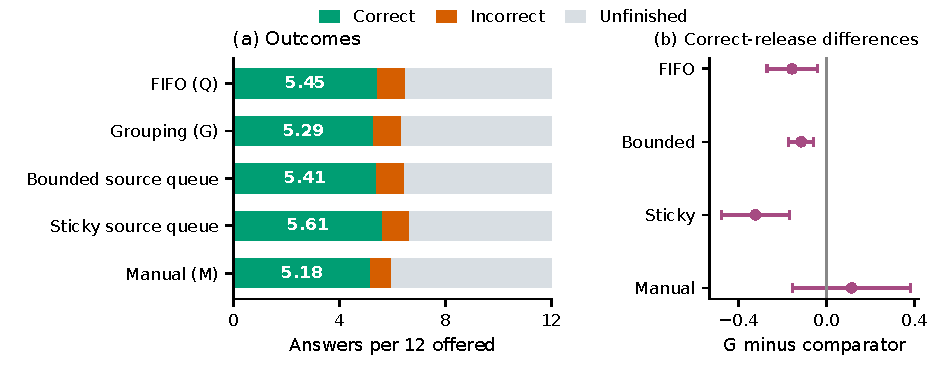
\includegraphics[width=\textwidth]{reference.pdf}
\caption{Simulated reference outcomes on real TAT-QA sources and saved drafts. (a) Correct, incorrect and unfinished answers per twelve offered. (b) G minus each comparator in correct releases; positive favors G. Means average three packets and 32 seeds; bars are 95\% Monte Carlo intervals over seed blocks, not participant uncertainty.}
\label{fig:reference}
\end{figure*}

\subsection{Design, Cutoff and Estimation}
The declared design contains 66 settings. The original setting crosses four orientation coefficients, three effectiveness profiles and two memory settings, giving 24 cells. Remaining cells use the higher profile and $S=25$, long memory and base costs unless varied. Twelve demand cells cross 6, 12, 24 or 36 offered questions with cutoffs of 270, 540 or 900 seconds. Six arrival cells cross interleaved or source-blocked order with two waves, a simultaneous burst, or arrivals spread over 480 seconds, using 24 questions. Six grouping-cost cells cross $S=5,25,75$ with costs of 0 or 12 seconds. Nine task-cost cells cross the three verification and manual costs. Nine carryover cells cross short, long or persistent memory with the three carryover probabilities.

For larger loads, packets are combined without duplicating questions. The six-question load uses the first three declared questions from each of two sources. The two-wave pattern places half the requests evenly over 0--20 seconds and the remainder over 180--200 seconds. In every scenario all offered tasks remain in the denominator. At the cutoff $H$, partial review time is charged, and an approval without completed release remains unfinished. Completion exactly at $H$ is accepted. Rejected, deferred, active and never-selected items all remain unfinished; none is counted as a correct completion.

Each cell uses three packet rotations, 32 independent Monte Carlo seeds (10000--10031) and five policies, giving $66\times3\times32\times5=31{,}680$ runs. Random draws are keyed by seed, question identifier, attempt and component. Matched policies therefore share potential difficulties and outcomes when taking the same path. Ordering can change carryover eligibility and which paths are reached.

For policy $p$, rotation $r$ and seed $b$, define
\begin{equation}
 Y_{p,r,b}=\frac{1}{N}\sum_{i=1}^{N} R_{i,p,r,b} C_{i,p,r,b}.
 \label{eq:outcome}
\end{equation}
Here $R$ indicates release of the current output version and $C$ its joint answer-and-scale correctness. The paired comparison first averages rotations,
\begin{equation}
 D_b=\frac{1}{3}\sum_{r=1}^{3}(Y_{G,r,b}-Y_{p,r,b}),\qquad
 \widehat\Delta=\frac{1}{32}\sum_{b=1}^{32}D_b.
 \label{eq:paired}
\end{equation}
Intervals are $\widehat\Delta\pm1.96\,s_D/\sqrt{32}$. Figures also show the equivalent difference in answers, $N\widehat\Delta$. These are normal Monte Carlo intervals conditional on the fixed sources and reviewer model. They quantify numerical precision, not variation among people or uncertainty about the behavioral assumptions. We report all designed settings, with no outcome-based retuning. Setting counts are not estimates of the prevalence of workplace conditions.

\begin{figure*}[t]
\centering
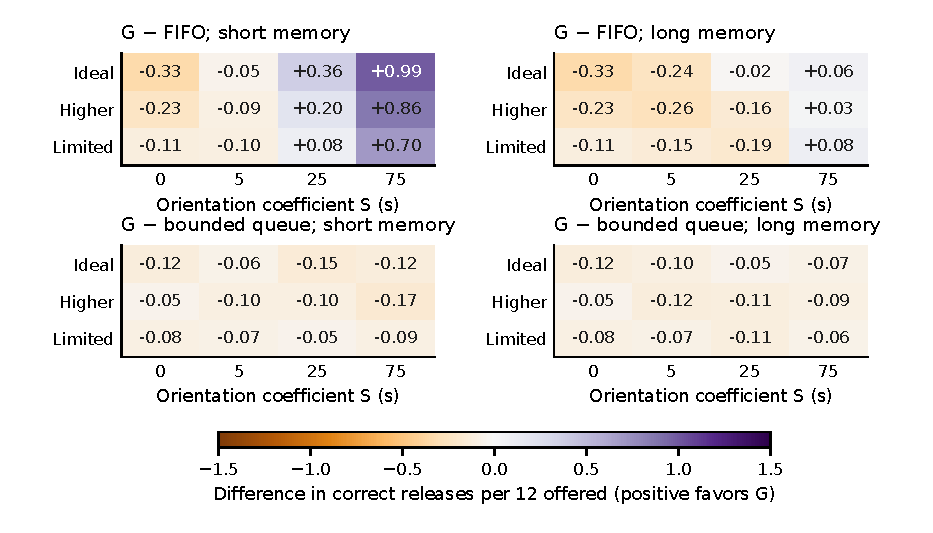
\includegraphics[width=\textwidth]{orientation.pdf}
\caption{Discrete simulated differences per twelve real-source questions and nine minutes, averaged across three rotations and 32 seeds. Columns vary orientation cost; panels vary memory and comparator. Reviewer profiles follow Table~\ref{tab:parameters}. The common zero-centered scale shows tested means without interpolation or human-population inference.}
\label{fig:orientation}
\end{figure*}

\section{RESULTS AND DESIGN IMPLICATIONS}
\label{sec:results}
\subsection{The Strongest Control Changes the Conclusion}
Figure~\ref{fig:reference} gives the reference comparison at twelve questions, nine minutes, $S=25$, long memory and higher effectiveness. Mean correct releases are 5.45 for Q, 5.29 for G, 5.41 for the bounded source queue, 5.61 for the sticky queue and 5.18 for M. Incorrect releases remain about one per block. More than five questions remain unfinished under every policy. The corresponding G--Q difference is $-0.156$ answers, with Monte Carlo interval $[-0.270,-0.043]$.\aicredit



The G--bounded-queue difference is $-0.115$ answers $[-0.170,-0.059]$, and G--sticky is $-0.323$ $[-0.477,-0.169]$. Across the complete grid, G is below the bounded queue in 62 setting means and tied in four. Three ties occur at zero grouping cost, where identity is built in. The fourth is an ample-capacity condition. Against FIFO, G has 24 favorable means, two ties and 40 unfavorable means; against the sticky queue, it has six favorable, one tied and 59 unfavorable means. These signs retain adverse conditions but do not define a global treatment effect over a naturally sampled population.

Mean orientation time is 69.86 seconds for Q, 61.06 for G and 61.86 for the bounded queue; G adds 10.72 seconds of grouping. Different completed task sets prevent interpreting these totals as a matched causal decomposition. G nevertheless reduces mean source switches from 6.71 to 2.48 without increasing correct releases. Switch counts alone are insufficient.

\subsection{When Reorientation Matters}
Figure~\ref{fig:orientation} exposes the operating region. At $S=25$ with the higher profile, G--Q is $+0.198$ answers $[0.081,0.315]$ with short memory, but $-0.156$ with long memory. Rapid loss of familiarity makes consecutive source use more valuable. When familiarity persists, FIFO retains much of the same context and grouping has less orientation time to save.



With $S=75$, short memory and higher effectiveness, the G--Q gain reaches $+0.865$ answers $[0.727,1.002]$. It is accompanied by an increase in incorrect releases from 0.688 to 0.833. Additional review capacity can release both more correct and more incorrect answers. The lower panels show that the bounded source-aware control still captures the selection benefit more economically.

Arrival structure also matters. With 24 questions in two waves, G--Q is $+0.583$ answers $[0.462,0.704]$ when sources interleave. Keeping each source's questions together reduces it to $-0.042$ $[-0.090,0.007]$. FIFO already reuses context in that order. A source-blocked workload therefore provides little additional opportunity for grouping, even though the cards are unchanged.

A simple conditional balance clarifies the mechanism. For the same attempted tasks, outcomes and non-orientation phases, the time made available by grouping is
\begin{equation}
 \Delta T = \sum_i(O_{Q,i}-O_{G,i})-n_g g,
 \label{eq:balance}
\end{equation}
where $n_g$ is the number of opened groups and $g$ their cost. Positive $\Delta T$ must still be sufficient to finish another decision and release before the cutoff. Changed selection can delay other requests, and an extra release can be wrong. Equation~\ref{eq:balance} is a model-based bookkeeping condition, not a measured law of attention or a guarantee of higher quality.

\begin{figure*}[t]
\centering
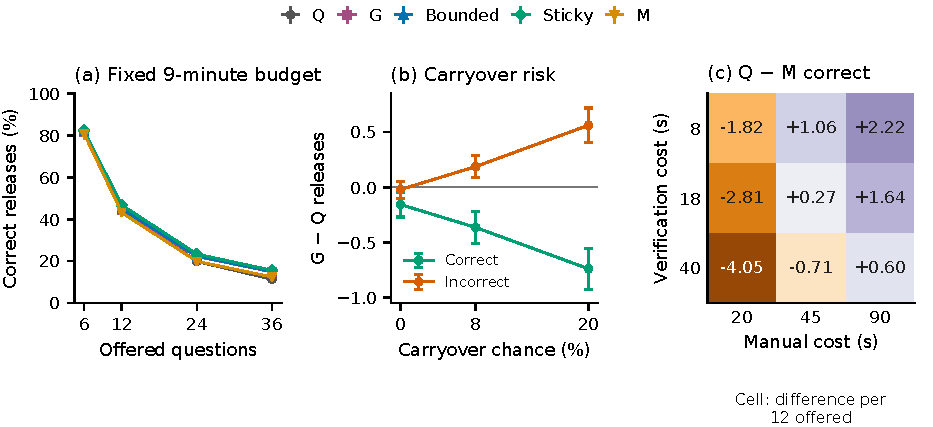
\includegraphics[width=\textwidth]{tradeoffs.pdf}
\caption{Assumption sensitivities using the same real-source question pool. (a) Simulated correct releases divided by all offered questions at a nine-minute cutoff; lines connect tested loads, not a fitted response curve. (b) Long-memory carryover scenarios, twelve offered, showing G--Q differences for correct and incorrect releases. Error bars in (a,b) are 95\% Monte Carlo intervals from 32 paired seed blocks, averaging three rotations. (c) Q--M correct-release differences per twelve offered as assumed base verification and manual-construction times vary; positive favors the draft-assisted FIFO queue. The cells are simulated, not measured review times or assistance effects.}
\label{fig:tradeoffs}
\end{figure*}

\subsection{Capacity, Carryover and Draft Usefulness}
Figure~\ref{fig:tradeoffs} separates three further limits. At a fixed nine-minute budget, increasing offered work reduces the correct-release fraction for every policy. With six questions and fifteen minutes, all four assisted policies have the same means: 5.031 correct, 0.938 incorrect and 0.031 unfinished. That is a low-contention tie under the model, not evidence of interface equivalence.



Carryover challenges an assumption that shared context only helps. With long memory and carryover probability 0.20, G--Q falls to $-0.740$ answers $[-0.925,-0.555]$. G's mean incorrect releases increase from 1.042 without carryover to 1.688. The corresponding Q means are 1.063 and 1.125. The model makes consecutive source use expose more requests to the same carryover mechanism. This identifies a failure condition worth observing, not an estimated frequency of human unit or assumption errors.

Poor drafts also create an assistance question independent of grouping. In the reference, Q--M is $+0.271$ correct answers $[-0.007,0.548]$. Both use FIFO, making this the cleaner modeled draft-availability comparison. If manual construction takes 20 base seconds and verification takes 40, Q--M becomes $-4.052$ answers. If manual construction takes 90 seconds and verification takes eight, it becomes $+2.219$. Detected-error repair still costs 45 seconds in these cells. Thus the initial mix of seven correct drafts, incorrect drafts and missing answers can either help or burden the reviewer depending on the cost of checking versus reconstructing them. Neither direction establishes what people will do.

The design implication is to retain simple source-aware navigation, report errors and outstanding work alongside throughput, and test draft usefulness against manual construction. Source organization must remain separate from answer authority: resolving one question is not permission to transfer its value, unit or interpretation to another.

\section{LIMITS AND HUMAN VALIDATION}
\label{sec:limits}
Workflow properties concern application state, not semantic correctness or comprehension. Tested interleavings do not establish reliability across arbitrary deployment failures. The simulation establishes conditional model consequences.\aicredit

The six reused contexts are not independently sampled organizations. Expertise, source ambiguity and learning across sessions are unmodeled. TAT-QA matching may penalize acceptable wording; future human adjudication must remain additional to official scores. Annotation-based corrections supply a success branch without measuring the reasoning needed to reach it. Agreement between answers is not an independent correctness check.

The uncalibrated familiarity equation has no effective source-size variation here. Fixed error profiles omit expertise-specific correlations and fine-grained interruption recovery. The model also lacks any visual-comprehension benefit or adaptive avoidance of grouping. Equal source reuse across policies is a necessary control, not a complete account of reading. More seeds cannot resolve these assumptions.

A frozen prospective study compares Q, G and M for twelve questions and nine minutes each, using disjoint source packets within participants and counterbalanced assignments. Admission controls are disabled. Participants are paired units for correct releases per offered question. Errors, unfinished work, source revisits, resumption, grouping use and self-reported workload and control remain separate outcomes. M tests draft usefulness. No participant observations have been collected.

Human validation must assess errors and source-aware choices in Q. Source openings are behavioral proxies; an uncertain difference is not equivalence.

\section{CONCLUSION}
Concurrent agent work needs explicit boundaries between generated, reviewed and released outputs. Our implemented workflow preserves evidence and versions during arrivals, keeps unfinished work accounted for, and supports source reuse without merging individual decisions.\aicredit

The simulation supports simple source-aware navigation as the necessary comparator for grouping. Grouping never exceeds that control in the 66 setting means. Our contribution is the specified oversight workflow and its conditional operating analysis. Whether grouped presentation helps people release more correct work remains an empirical question.

\section*{AI ASSISTANCE DISCLOSURE}
Codex assisted all prose, code, analyses, figures and evidence checks \cite{codex}. Reviewer outcomes are simulated; no participant data were generated. Authors retain responsibility for the submission.

{\small
\begin{thebibliography}{9}
\bibitem[Epperson et~al., 2025]{agdebugger}
Epperson, W., Bansal, G., Dibia, V., Fourney, A., Gerrits, J., Zhu, E., and Amershi, S. (2025).
Interactive debugging and steering of multi-agent AI systems.
In \emph{Proceedings of CHI}. ACM.
\doi{10.1145/3706598.3713581}.

\bibitem[Iqbal and Horvitz, 2007]{iqbal}
Iqbal, S.~T. and Horvitz, E. (2007).
Disruption and recovery of computing tasks: Field study, analysis, and directions.
In \emph{Proceedings of CHI}, pages 677--686. ACM.
\doi{10.1145/1240624.1240730}.

\bibitem[OpenAI, 2026]{codex}
OpenAI (2026). Codex. AI development and drafting tool.
\url{https://openai.com/codex/}. Accessed September 2026.

\bibitem[Potts and Kovalyov, 2000]{potts}
Potts, C.~N. and Kovalyov, M.~Y. (2000).
Scheduling with batching: A review.
\emph{European Journal of Operational Research}, 120(2):228--249.
\doi{10.1016/S0377-2217(99)00153-8}.

\bibitem[Zhao et~al., 2026]{agentgui}
Zhao, X., Sohn, J., Zheng, Q., and Moor, M. (2026).
AgentGUI: An interface for observing and steering long-running AI agents.
\emph{arXiv preprint}, 2607.26300v2.
\url{https://arxiv.org/abs/2607.26300}.

\bibitem[Zhu et~al., 2021]{tatqa}
Zhu, F., Lei, W., Huang, Y., Wang, C., Zhang, S., Lv, J., Feng, F., and Chua, T.-S. (2021).
TAT-QA: A question answering benchmark on a hybrid of tabular and textual content in finance.
In \emph{Proceedings of ACL-IJCNLP}, pages 3277--3287.
\doi{10.18653/v1/2021.acl-long.254}.
\end{thebibliography}
}
\end{document}
